\documentclass[a4paper,12pt]{article}
\usepackage[utf8]{inputenc}
\usepackage{graphicx}
\usepackage{hyperref}
\usepackage{amsmath, amssymb}
\usepackage{authblk}
\usepackage{pdfpages}

\title{SustainCity: \\ The Future of Adaptive Urban Movement \\ v 1.0.1}
\author[1]{Giovanni La Gioia}
\vspace{0.5cm} % Space between authors
\author[2]{Luca Leonzio}
\vspace{0.5cm}
\author[3]{Matteo Parimbelli}
\vspace{0.5cm}
\author[4]{Serena Tolla}
\affil[1,2,3,4]{Politecnico di Milano}
\date{Last update: \today}

\begin{document}
\maketitle
\vspace{2cm}
\begin{center}
    
\includegraphics[width=0.6\textwidth]{diagrams/SustainCity_logo.png}
\end{center}
\newpage
\tableofcontents
\clearpage
\newpage

% SECTION 1 - The Project and Its Goals
\section{The Project and Its Goals}
The following describes the \textbf{SustainCity} project and its goals to be achieved, developed as part of the \textbf{Software Engineering for HPC} course. We structured this first section into three key parts:
\begin{itemize}
    \item The \textbf{Preface}, introducing the broader environmental and urban challenges motivating this project.
    \item The \textbf{Problem Statement}, describing in detail the technical and society issues to be addressed.
    \item The \textbf{Project Goals}, outlining the core functionalities and expected outcomes.
\end{itemize}

\subsection*{Preface}
Two urgent global concerns are environmental sustainability and climate change; because of air pollution and greenhouse gas emissions, transportation - especially urban commuting - worsens those issues. 
\\ The objective of the SustainCity project is to face urban mobility challenges through real-time traffic management, event-driven optimizations, and public transport coordination. 
\\ To address these concerns, the project integrates traffic monitoring, event planning, and transport analytics into an adaptive system capable of creating data-driven recommendations for real-time city infrastructure improvements. 
\\ Thanks to these system recommendations, urban commuting can be drastically reduced, improving both citizens’ well-being and environmental sustainability.

\subsection*{Problem Statement}
The \textbf{SustainCity} system aims to optimize urban traffic using three key strategies:
\begin{itemize}
    \item \textbf{Real-time Traffic Optimization (Type1 Actions)} 
    The system continuously adapts traffic light timings using real-time congestion data to optimize flow.  
    \item \textbf{Long-term Traffic Pattern Analysis (Type2 Actions)}  
    The system analyzes daily congestion patterns to recommend permanent adjustments, such as one-way street configurations, adaptive traffic signal schedules, and public transport optimizations.
    \item \textbf{Event-driven Traffic Management (Type3 Actions)}
    SustainCity monitors city event feeds (e.g., concerts, fairs, sports games) and adjusts road and transport infrastructure dynamically to reduce congestion during high-footfall gatherings.
\end{itemize}

\noindent Additionally, SustainCity generates \textbf{reports for urban planners and citizens}:
\begin{itemize}
    \item \textbf{Daily Reports}: Summarizing average traffic flows and actions taken (Type1).
    \item \textbf{Yearly Reports}: Documenting major infrastructure proposals (Type2, Type3) and their implementation status (accepted/rejected).
\end{itemize}

\noindent To accomplish these goals, we can rely on the following elements: 
\begin{itemize}
    \item A preexisting infrastructure offering sensors that measure the number of seconds cars need to cross each intersection. This infrastructure is developed according to the event-based style. All sensors periodically publish the data they have acquired on a message bus. 
    \item A microservice offering information about public transport schedules. In particular, this microservice offers the following operations: 
    \begin{itemize} 
        \item \textbf{getScheduleByStreet}: Given the name of a street, it returns the timetable of all stops present on that street. 
        \item \textbf{getScheduleByLine}: Given the number of a specific line, it returns the complete timetable for that line.   
    \end{itemize}
    \item A news channel that transmits information about the events in the city as soon as they are planned.
\end{itemize}

\subsection*{Project Goals}
Our main goal was to develop a software system that creates efficient, sustainable urban transport solutions by providing data-driven recommendations. Therefore, the document aims to meet two objectives: 
\begin{itemize}
    \item Ensuring all functional and technical requirements are met.
    \item Designing a scalable, efficient, and well-structured urban-mobility solution.
\end{itemize}

\newpage

% SECTION 2 - Requirement Analysis
\section{Requirement Analysis}
\subsection{Relevant Human and Non-Human Actors}
Let's begin by examining the \textit{human actors} involved in this system first:
\begin{itemize}
    \item \textbf{Traffic Engineers} (Type1): They supervise and verify the correct functioning of the automatic traffic light regulation system. They take action in the event of malfunction, validate traffic management strategies, and analyze logs for future improvements.
    \item \textbf{Urban Area Manager} (Type1, Type2, Type3): They are responsible for overseeing urban infrastructure, long-term policies and constraints related to dynamic traffic light regulation. They also evaluate traffic optimization proposals and approve or reject recommendations related to traffic configurations, transportation scheduling, and road management. Their decisions directly impact the effectiveness of SustainCity's long-term strategies.
    \item \textbf{City Planners and Officials} (Type 1, Type2, Type3): Work alongside \textbf{Urban Area Managers} to assess traffic data reports, evaluate permanent infrastructure adaptations, and implement policy changes based on recommendations. They ensure that adjustments are in accordance with environmental and urban regulations. They may also be involved in the approval and monitoring of automated traffic regulation systems.
    \item \textbf{Citizens}(Type1, Type2, Type3): Although not actively involved in the system’s technical workings, they are end-users who benefit from improved traffic conditions, congestion reduction, and optimized public transport schedules. They receive notifications through city mobility platforms, public dashboards, transport apps, and digital road signs.
\end{itemize}
\noindent On the other hand, there are also several \textit{non-human actors} needed to ensure the system operates efficiently and delivers accurate data-driven insights:
\begin{itemize}
    \item \textbf{Traffic Management System} (Type1, Type2, Type3): Acts as the core analytical component by collecting, processing, and interpreting data from various sources, such as traffic sensors. This actor continuously monitors daily traffic flows, identifies congestion hot spots, and detects recurring traffic patterns that could benefit from optimization.
    \item \textbf{Public Transport Microservice} (Type2, Type3): Provides comprehensive and real-time public transport schedules. By integrating this microservice, the system can propose modifications to transport schedules, aligning them with identified traffic patterns to optimize commuter convenience and reduce congestion.
    \item \textbf{Sensors} (Type1, Type2, Type3): Physical devices deployed at intersections and major roadways; these actors gather real-time data about traffic conditions. Accurate and timely sensor data is foundational, enabling the system to analyze traffic patterns and propose meaningful optimizations reliably.
    \item \textbf{Event Monitoring System} (Type3): Detects and transmits event schedules (concerts, sports games, fairs), triggering event-driven traffic adjustments and real-time mobility recommendations. It works closely with the \textbf{Traffic Management System} and \textbf{Public Transport Microservice} to prevent congestion.
    \item \textbf{Notification System} (Type1, Type2, Type3): A critical component for disseminating structured reports and real-time alerts to all relevant actors. It ensures that traffic management decisions — whether real-time, event-driven, or long-term — are properly communicated to all relevant stakeholders.
\end{itemize}

\newpage

\section{Use Cases}
The following use cases describe how the system interacts with traffic data, urban managers, and external events to achieve its objectives. Each use case type corresponds to a specific level of system autonomy and decision-making: Type1 actions are fully automated, Type2 involve semi-automated analysis with human validation, and Type3 relate to exceptional or event-driven scenarios requiring coordinated interventions. The use cases are organized into tables for clarity.
\\ We have also decided to analyze only the three most important use cases for each type of action in order to gain a better understanding of them.

\subsection{Type1 Use Cases}
\begin{table}[h!]
\centering
\begin{tabular}{|p{4.5cm}|p{8.5cm}|}
\hline
\textbf{Use Case} & \textbf{Description} \\
\hline
Real-Time Traffic Monitoring & The system continuously receives data from traffic sensors at key intersections, monitoring vehicle wait times and traffic density. \\
\hline
Dynamic Light Adjustment Decision & Based on thresholds or patterns, the system autonomously decides to alter green light durations using predefined rules or adaptive algorithms. \\
\hline
Actuation of Traffic Light Changes & Once a decision is made, the system dispatches updated timing configurations to traffic lights for short-term application. \\
\hline
\end{tabular}
\caption{Type1 Use Cases}
\end{table}

\subsubsection*{Use Case 1: Real-Time Traffic Monitoring}
\textbf{Primary Actors}: Traffic Sensors \\
\textbf{Supporting Actors}: Traffic Management System \\
\textbf{Use case flow}: 
\begin{enumerate}
    \item \textit{Collect Data} Traffic sensors continuously measure real-time vehicle wait times and traffic density at intersections and publish this data on the event bus.
    \item \textit{Receive and Process Data} The Traffic Management System continuously receives and validates incoming sensor data, checking for data consistency and accuracy.
    \item \textit{Store and Document Data} The processed data is stored internally for immediate access by other modules within the Traffic Management System.
\end{enumerate}
\textbf{Assumptions}: 
\begin{itemize}
    \item Traffic Sensors  fully operational
    \item The event bus system is reliable and timely \\
\end{itemize}
\textbf{Requirements}: FR1, FR2 (See Functional Requirements section)
\\
\begin{figure}[h]
    \centering
    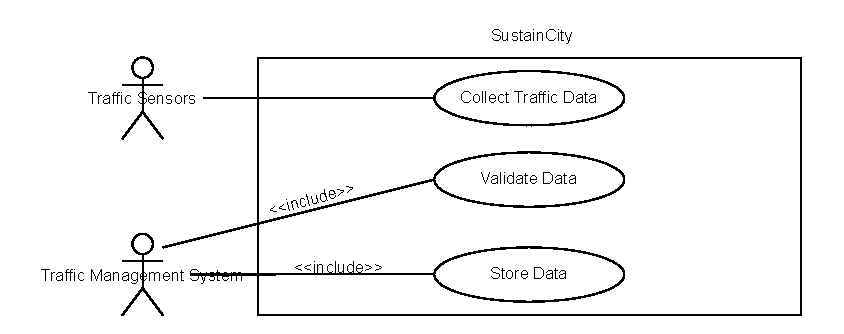
\includegraphics[width=0.8\textwidth]{diagrams/Real-Time_Traffic_Monitoring.drawio.pdf}
    \caption{Use Case 1 Diagram, Real-Time Traffic Monitoring}
    \label{fig:Real-Time_Traffic_Monitoring.drawio}
\end{figure}
\\

\subsubsection*{Use Case 2: Dynamic Light Adjustment Decision}
\textbf{Primary Actors}: Traffic Management System \\
\textbf{Supporting Actors}: Traffic Sensors, Notification System \\
\textbf{Use case flow}: 
\begin{enumerate}
    \item \textit{Evaluate Traffic Conditions} Traffic Management System evaluates received sensor data to identify congestion or imbalance between intersecting roads.
    \item \textit{Decision Making} Based on predefined thresholds and adaptive algorithms, the system autonomously decides if traffic light timing adjustments are necessary.
    \item \textit{Prepare Adjustment Instructions} System formulates the specific adjustment parameters required for each affected intersection.
\end{enumerate}
\textbf{Assumptions}: 
\begin{itemize}
    \item Accuracy and Reliability of pre-defined thresholds and adaptive algorithm
    \item Real-time processing capabilities exist within the system
\end{itemize} 
\textbf{Requirements}: FR3
\\
\begin{figure}[h]
    \centering
    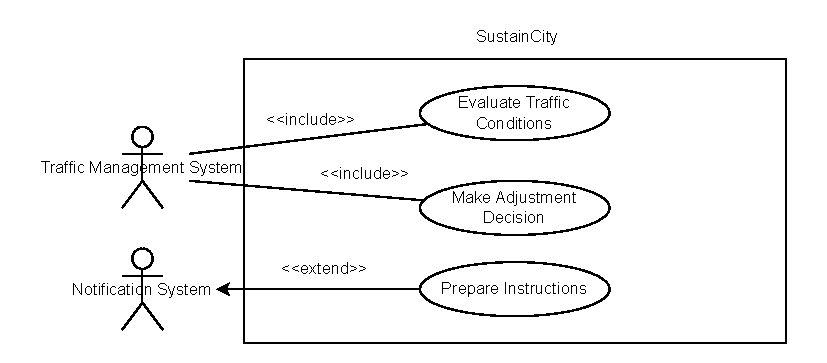
\includegraphics[width=0.8\textwidth]{diagrams/Dynamic_Light_Adjustment_Decision.drawio.pdf}
    \caption{Use Case 2 Diagram, Dynamic Light Adjustment Decision}
    \label{fig:Dynamic_Light_Adjustment_Decision.drawio}
\end{figure}
\\

\subsubsection*{Use Case 3: Actuation of Traffic Light Changes}
\textbf{Primary Actors}: Traffic Management System \\
\textbf{Supporting Actors}: Traffic Controllers, Notification System \\
\textbf{Use case flow}: 
\begin{enumerate}
    \item \textit{Dispatch Adjustment Commands} System sends calculated timing configurations directly to the traffic controllers managing the physical lights.
    \item \textit{Apply Configuration Immediately} Traffic controllers immediately apply the new timing settings without human intervention.
    \item \textit{Log Action} Traffic Management System logs the applied changes, including time of application, intersections affected, and rationale for transparency and audit purposes.
    \item \textit{Public Notification} Notification System optionally communicates any critical short-term adjustments to commuters via dashboards if necessary.
\end{enumerate}
\textbf{Assumptions}: 
\begin{itemize}
    \item Reliability and uninterrupted communication between the management system and traffic controllers.
\end{itemize}
\textbf{Requirements}: FR3, FR8, FR9, FR10
\\
\begin{figure}[h]
    \centering
    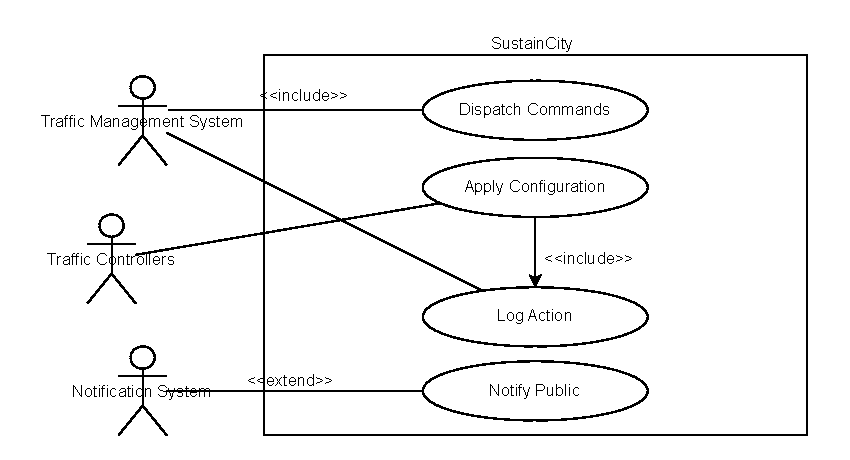
\includegraphics[width=0.8\textwidth]{diagrams/Actuation_of_Traffic_Light_Changes.drawio.pdf}
    \caption{Use Case 3 Diagram, Actuation of Traffic Light Changes}
    \label{fig:Actuation_of_Traffic_Light_Changes.drawio}
\end{figure}
\\


\newpage

\subsection{Type2 Use Cases}
\begin{table}[h!]
\centering
\begin{tabular}{|p{4.5cm}|p{8.5cm}|}
\hline
\textbf{Use Case} & \textbf{Description} \\
\hline
Traffic Pattern and Public Transport Analysis & The system processes daily traffic and public transport data to detect recurring congestion patterns, bottlenecks, or inefficiencies. \\
\hline
Suggest Optimizations & Based on analysis, the system recommends traffic light adjustments, road direction changes, and transit schedule modifications. \\
\hline
Review and Apply Changes & Urban area managers review and approve or reject system-generated suggestions, implementing selected actions. All modifications are published on User App and maps are modificated. \\
\hline
\end{tabular}
\caption{Type2 Use Cases}
\end{table}

\subsubsection*{Use Case 1: Traffic Pattern and Public Transport Analysis}
\textbf{Primary Actors}: Traffic Sensors, Public Transport Microservice \\
\textbf{Supporting Actors}: Traffic Management System \\ 
\textbf{Use case flow}: 
\begin{enumerate}
    \item \textit{Collect Data} Traffic sensors and Public transport microservice continuously measure the traffic and public transport conditions and constantly publish this data on the event bus.
    \item \textit{Process Traffic Data} The system processes incoming sensor data, filtering out anomalies and organizing it into usable information.
    \item \textit{Store Analysis Results} The data collected are stored internally for use by the Optimization Engine. The data provided must be usable for the Traffic Management System.
\end{enumerate}
\textbf{Assumptions}: 
\begin{itemize}
    \item Traffic sensors and Public Transport Microservice always working with enough storage.
\end{itemize}
\textbf{Requirements}: FR1, FR2
\\
\begin{figure}[h]
    \centering
    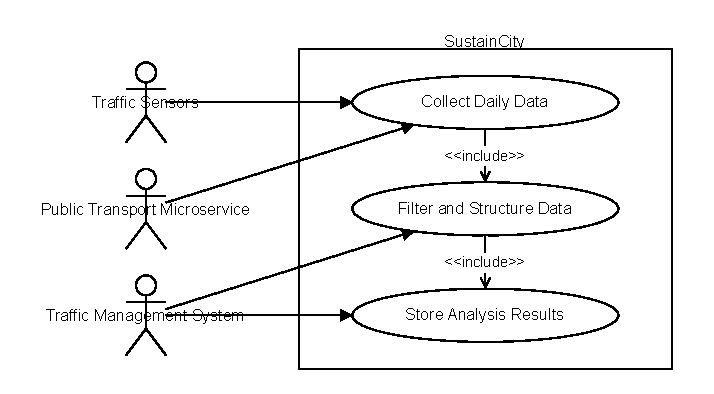
\includegraphics[width=0.8\textwidth]{diagrams/Traffic_Pattern_and_Public_Transport_Analysis.drawio.pdf}
    \caption{Use Case 1 Diagram, Traffic Pattern and Public Transport Analysis}
    \label{fig:Traffic_Pattern_and_Public_Transport_Analysis.drawio}
\end{figure}
\\

\subsubsection*{Use Case 2: Suggest Optimizations}
\textbf{Primary Actors}: Traffic Management System \\
\textbf{Supporting Actors}:  Urban Area, Traffic Sensors, Public Transport Microservice \\
\textbf{Use case flow}: 
\begin{enumerate}
    \item \textit{Retrieve Analysis Results}
    The Optimization Engine retrieves combined traffic pattern and public transport data results previously generated by the sensors and the microservice.
    \item \textit{Data refinement} The Traffic Management System apply techniques in order to have data ready to be processed for Machine Learning techniques both for Supervised and Unsupervised data.
    \item \textit{Generate Optimization Recommendations} The system generates a detailed list of specific, actionable optimization suggestions, including: recommended directional changes for particular road segments, proposed timetable modifications for bus and tram services.
    \item \textit{Prioritize and Store Recommendations} The system prioritizes and store the generated recommendations based on expected effectiveness, feasibility, and urgency, forming a ranked list.
    \item \textit{Present Recommendations to Urban Area Manager} The Optimization Engine makes recommendations accessible through the Urban Area Manager Interface for further review and decision-making. The optimizations suggested must be readable for Urban Area Manager.
\end{enumerate}
\textbf{Assumptions}: 
\begin{itemize}
    \item Traffic Management System can perform Machine Learning techniques and has enough computational power
    \item Data provided by the sensors are ready to be used
    \item Traffic Management System provides optimization report for Urban Area Manager.
\end{itemize}
\textbf{Requirements}: FR4
\\
\begin{figure}[h]
    \centering
    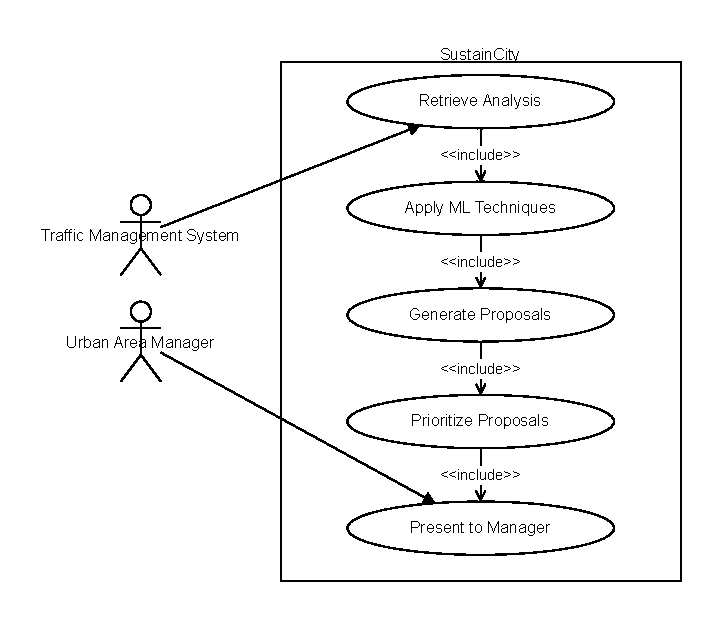
\includegraphics[width=0.8\textwidth]{diagrams/Suggest_Optimizations.drawio.pdf}
    \caption{Use Case 2 Diagram, Suggest Optimizations}
    \label{fig:Suggest_Optimizations.drawio}
\end{figure}
\\

\subsubsection*{Use Case 3: Review and Apply Changes}
\textbf{Primary Actors}: Urban Area Manager, City Planners \\
\textbf{Supporting Actors}: Traffic Management System \\ 
\textbf{Use case flow}: 
\begin{enumerate}
    \item \textit{Access Optimization Recommendations} Urban Area Manager accesses the optimization suggestions presented by the Optimization Engine via the Management Dashboard.
    \item \textit{Review Optimization Suggestions} Manager and City Planners evaluates each optimization suggestion carefully, considering feasibility, expected benefits, potential impact, and citizen feedback previously received.
    \item \textit{Approve or Reject Suggestions} Manager decides whether to approve or reject each suggestion individually.
    \item \textit{Implement Approved Changes} For each approved optimization, road direction changes are physically implemented and updated in traffic signs.
    Public transit schedules are updated and communicated to the Public Transport Microservice.
    \item \textit{Update City Maps and User App} All implemented changes are reflected promptly in: Official city maps.
    The User App, ensures citizens are immediately informed about modifications.
    \item \textit{Publish Modification Reports} The Reporting Module generates and publishes a detailed public report via the User App, informing citizens about changes and their expected benefits.
\end{enumerate}
\textbf{Assumptions}: 
\begin{itemize}
    \item The User App and city map services are operational and capable of real-time updates.
\end{itemize}
\textbf{Requirements}: FR5, FR10
\\
\newpage
\begin{figure}[h]
    \centering
    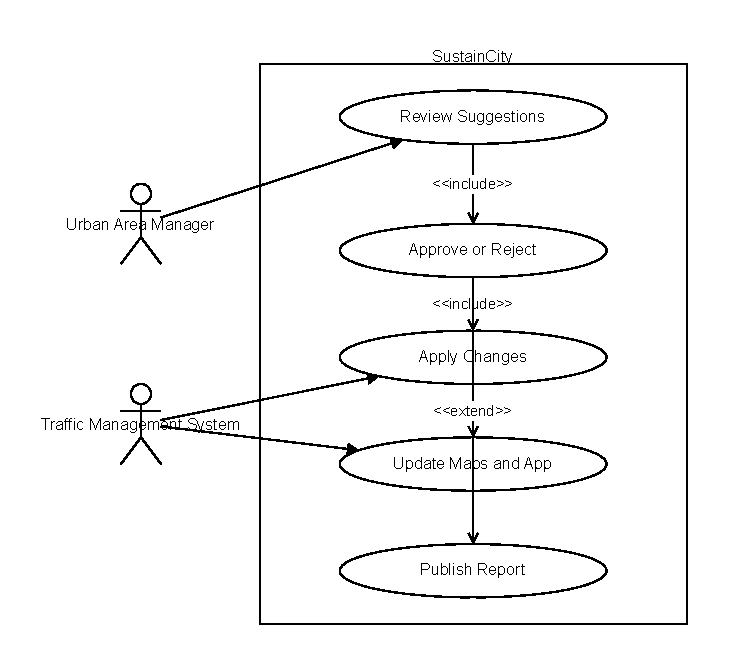
\includegraphics[width=0.8\textwidth]{diagrams/Review_and_Apply_Changes.drawio.pdf}
    \caption{Use Case 3 Diagram, Review and Apply Changes}
    \label{fig:Review_and_Apply_Changes.drawio}
\end{figure}


\newpage

\subsection{Type3 Use Cases}
\begin{table}[h!]
\centering
\begin{tabular}{|p{4.5cm}|p{8.5cm}|}
\hline
\textbf{Use Case} & \textbf{Description} \\
\hline
Traffic Disruption Forecasting & It predicts congestion using event data, historical trends, and real-time sensor input, enabling preemptive planning. \\
\hline
Dynamic Mobility Adaptation & The system adapts traffic lights, road usage, and public transport routes in response to forecasts. \\
\hline
Public Engagement and Notification & Citizens are informed through mobile apps and dashboards about changes, alternate routes, and delays. \\
\hline
\end{tabular}
\caption{Type3 Use Cases}
\end{table}

\subsubsection*{Use Case 1: Traffic Disruption Forecasting}
\textbf{Primary Actors}: Traffic Management System, Event Monitoring System \\
\textbf{Supporting Actors}: Traffic Sensors, Public Transport Microservices \\
\textbf{Use case flow}: 
\begin{enumerate}
    \item \textit{Event Detection} The Event Monitoring System identifies a planned city event (e.g., concert, fair, sports match) and transmits details (location, duration, expected attendance).
    \item \textit{Traffic Impact Analysis} The Traffic Management System retrieves historical congestion data for similar events, comparing it with real-time traffic conditions to predict disruption levels.
    \item \textit{Congestion Prediction Modeling} AI-driven algorithms forecast expected delays and bottlenecks, generating a predictive traffic model.
    \item \textit{Risk Categorization} he system classifies events by severity (minor, moderate, high-impact) based on anticipated congestion and traffic complexity.
    \item \textit{Decision Preparation} The predictive findings are stored for use by Dynamic Mobility Adaptation and Public Notification workflows.
\end{enumerate}
\textbf{Assumptions}: 
\begin{itemize}
    \item Event Monitoring System continuously provides real-time updates on planned city events.
    \item Historical traffic data is available and reliable for prediction accuracy.
\end{itemize}
\textbf{Requirements}: FR2, FR6
\\
\begin{figure}[h]
    \centering
    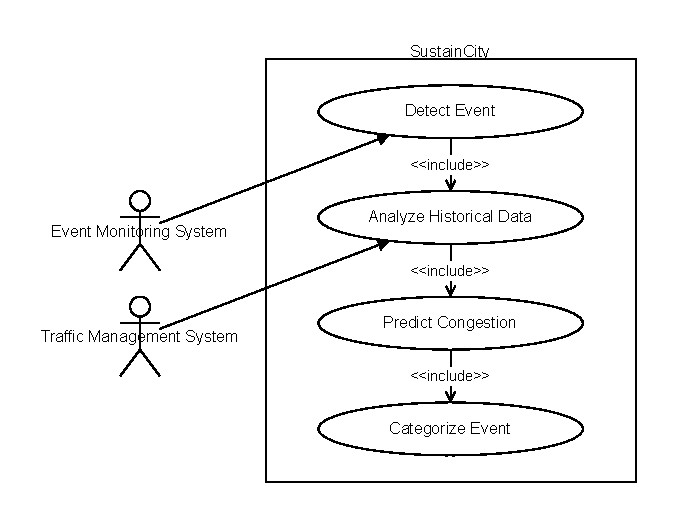
\includegraphics[width=0.8\textwidth]{diagrams/Traffic_Disruption_Forecasting.drawio.pdf}
    \caption{Use Case 1 Diagram, Traffic Disruption Forecasting}
    \label{fig:Traffic_Disruption_Forecasting.drawio}
\end{figure}
\\

\subsubsection*{Use Case 2: Dynamic Mobility Adaptation}
\textbf{Primary Actors}: Traffic Management System \\
\textbf{Supporting Actors}: Traffic Sensors, Public Transport Microservices, Notification System \\
\textbf{Use case flow}: 
\begin{enumerate}
    \item \textit{Retrieve Congestion Forecast} Traffic Management System accesses predicted event-driven congestion analysis results.
    \item \textit{Compute Response Strategy} System generates adaptive changes, including traffic light timing adjustments, altered lane usage, and public transport rerouting.
    \item \textit{Validate Adaptations} Proposed mobility adjustments are reviewed to ensure feasibility and alignment with broader urban management strategies.
    \item \textit{Implement Changes} Traffic lights, road usage, and transport routes are updated dynamically based on final validation.
    \item \textit{Citizen Notification} Commuters are informed of temporary road modifications through digital dashboards and mobile apps.
\end{enumerate}
\textbf{Assumptions}: 
\begin{itemize}
    \item Traffic controllers are capable of receiving and implementing adaptive changes in near-real time.
    \item Commuters actively engage with public notifications to adjust their travel plans accordingly.
\end{itemize}
\textbf{Requirements}: FR3, FR7
\\
\begin{figure}[h]
    \centering
    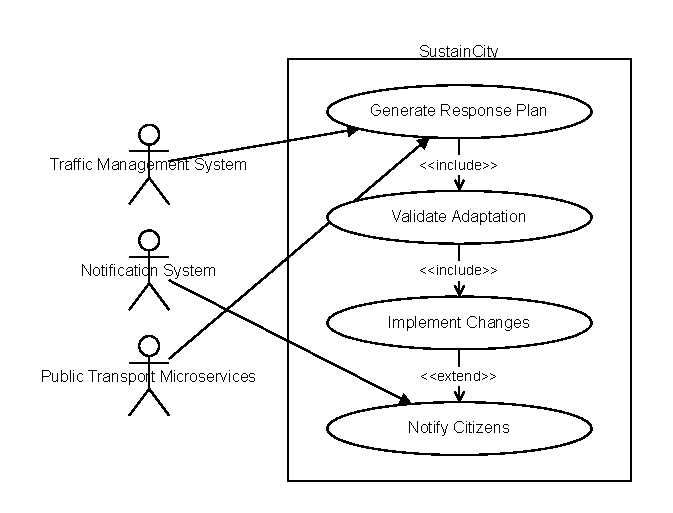
\includegraphics[width=0.8\textwidth]{diagrams/Dynamic_Mobility_Adaptation.drawio.pdf}
    \caption{Use Case 2 Diagram, Dynamic Mobility Adaptation}
    \label{fig:Dynamic_Mobility_Adaptation.drawio}
\end{figure}
\\

\subsubsection*{Use Case 3: Public Engagement and Notification}
\textbf{Primary Actors}: Notification System \\
\textbf{Supporting Actors}: Traffic Management System, Urban Area Manager\\
\textbf{Use case flow}: 
\begin{enumerate}
    \item \textit{Generate Citizen Alerts}  Notification System prepares targeted messages regarding upcoming event-driven mobility changes.
    \item \textit{Select Communication Channels} System chooses optimal dissemination platforms (city mobility apps, transport displays, public dashboards)
    \item \textit{Distribute Information} Alerts are broadcast across multiple channels, ensuring maximum commuter reach.
    \item \textit{Citizen Interaction Tracking} System monitors engagement metrics (view rates, clicks) to assess notification effectiveness.
    \item \textit{Feedback Loop}  Public responses are logged and analyzed to refine future engagement strategies.
\end{enumerate}
\textbf{Assumptions}: 
\begin{itemize}
    \item Citizens actively use digital mobility platforms to stay informed.
    \item Public dashboards and apps are capable of delivering real-time updates.
\end{itemize}
\textbf{Requirements}: FR10, FR11
\\
\newpage

\begin{figure}[h]
    \centering
    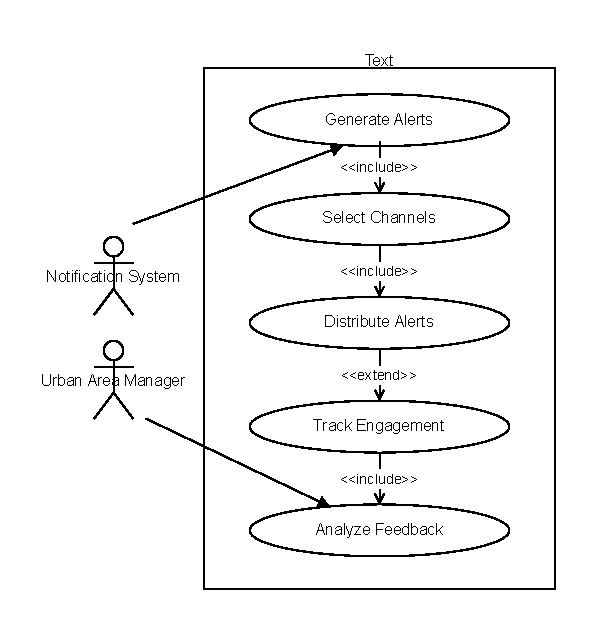
\includegraphics[width=0.8\textwidth]{diagrams/Public_Engagement_and_Notification.drawio.pdf}
    \caption{Use Case 3 Diagram, Public Engagement and Notification}
    \label{fig:Public_Engagement_and_Notification.drawio}
\end{figure}


\newpage

\subsection{Domain Assumptions}

The correct operation of the system is based on the following cross-cutting assumptions, organized by thematic area and referencing the relevant use case types (Type1, Type2, Type3).

\begin{itemize}

    \item \textit{Sensor Infrastructure Reliability} (Type1, Type2, Type3): The system assumes that traffic sensors deployed across the city, especially at intersections and major roads, are consistently operational. These sensors provide essential real-time data for adaptive traffic light control (Type1), daily traffic pattern analysis (Type2), and congestion prediction during large events (Type3).

    \item \textit{Autonomous Traffic Light Control} (Type1): The system is authorized to autonomously adjust traffic light timings based on real-time sensor data, without prior approval. These adjustments target immediate traffic imbalances and are the foundation for reactive traffic management.

    \item \textit{Urban Area Manager Oversight} (Type2, Type3): Although the system can autonomously manage traffic lights, larger changes, such as reconfiguring roads or updating public transport schedules, require approval from urban area managers. Their role ensures that data-driven suggestions align with long-term urban planning.

    \item \textit{Public Transport Data Availability} (Type2, Type3): The system relies on up-to-date access to the public transport microservice, providing accurate timetables and real-time data. This supports both optimization of daily operations (Type2) and event-based rerouting (Type3).

    \item \textit{Event Data Feeds} (Type3): The system assumes continuous access to official city event schedules, allowing early detection of high-impact gatherings and preparation of mobility strategies accordingly.

    \item \textit{Inter-System Communication} (Type 1, Type 2, Type 3): Reliable and stable network infrastructure is essential to enable seamless communication among the traffic management system, microservices, event monitoring module, sensors, and urban manager interfaces. Delays or failures in communication could hinder real-time reactions (Type1), the generation of optimization proposals (Type2), and the coordination of event-driven responses (Type3).

    \item \textit{Logging and Traceability} (Type1, Type2): All system actions, especially autonomous interventions and proposed suggestions, are assumed to be automatically logged. This ensures accountability, supports auditing by human actors, and enables future analysis.

    \item \textit{Real-Time Processing Capabilities} (Type1, Type3): The system is assumed to be capable of real-time or near-real-time decision-making, which is essential for reacting to live traffic conditions (Type1) and dynamically adapting to disruptions during events (Type3).

    \item \textit{Public Awareness and Engagement} (Type3): For event-driven adjustments to be effective, it is assumed that citizens actively consult and respond to the notifications distributed through the system. Informed commuters are critical to mitigating congestion during critical timeframes.
    
\end{itemize}

\newpage

\subsection{Requirements}

\subsubsection{Functional Requirements}

This section consolidates and explains the Functional Requirements (FRs) identified within the use cases, explicitly mapping each FR to the corresponding use cases. \\

\begin{itemize}
\item \textbf{FR1: Real-Time Data Collection} \\
The system must continuously collect real-time data from traffic sensors and public transport microservices. This ensures accurate monitoring and effective decision-making. \\
\textbf{Associated Use Cases:}
\begin{itemize}
\item Type1: Real-Time Traffic Monitoring
\item Type2: Traffic Pattern and Public Transport Analysis
\end{itemize}
\item \textbf{FR2: Accurate Data Processing} \\
The system must ensure the accuracy and reliability of data collected from sensors and microservices. The integrity of this data is essential for reliable system operations. \\
\textbf{Associated Use Cases:}
\begin{itemize}
\item Type1: Real-Time Traffic Monitoring
\item Type2: Traffic Pattern and Public Transport Analysis
\item Type3: Traffic Disruption Forecasting
\end{itemize}
\item \textbf{FR3: Autonomous Decision-Making} \\
The system must autonomously identify traffic imbalances and dynamically decide adjustments, such as modifying traffic light timings or traffic configurations based on real-time data. \\
\textbf{Associated Use Cases:}
\begin{itemize}
\item Type1: Dynamic Light Adjustment Decision, Actuation of Traffic Light Changes
\item Type3: Dynamic Mobility Adaptation
\end{itemize}

\item \textbf{FR4: Optimization Recommendations Generation} \\
The system must generate clear and actionable optimization recommendations based on traffic analysis, including adjustments in traffic signals, road direction changes, and public transportation schedules. \\
\textbf{Associated Use Cases:}
\begin{itemize}
\item Type2: Suggest Optimizations
\end{itemize}

\item \textbf{FR5: Recommendation Management} \\
The system must enable urban area managers to explicitly approve or reject optimization suggestions via an intuitive dashboard interface. \\
\textbf{Associated Use Cases:}
\begin{itemize}
\item Type2: Review and Apply Changes
\item Type3: Approval Workflow Management
\end{itemize}

\item \textbf{FR6: Event-driven Congestion Forecasting} \\
AI-driven forecasting models must predict congestion levels and categorize event impacts to facilitate preemptive traffic management planning. \\
\textbf{Associated Use Cases:}
\begin{itemize}
\item Type3: Traffic Disruption Forecasting
\end{itemize}

\item \textbf{FR7: Real-Time Public Transport Coordination} \\
The system must dynamically adjust public transport availability to meet event-driven demands and minimize congestion. \\
\textbf{Associated Use Cases:}
\begin{itemize}
\item Type3: Dynamic Mobility Adaptation
\end{itemize}

\item \textbf{FR8: Immediate Application of Changes} \\
The system must autonomously dispatch and immediately apply traffic configuration changes without manual intervention to promptly address identified issues. \\
\textbf{Associated Use Cases:}
\begin{itemize}
\item Type1: Actuation of Traffic Light Changes
\end{itemize}

\item \textbf{FR9: Comprehensive Logging} \\
All actions, decisions, and applied changes must be comprehensively logged with timestamps, intersections affected, and rationale for auditing purposes and transparency. \\
\textbf{Associated Use Cases:}
\begin{itemize}
\item Type1: Actuation of Traffic Light Changes
\end{itemize}

\item \textbf{FR10: Citizen Notification and Engagement} \\
The system must distribute clear, timely, and actionable notifications through multiple digital platforms, engaging citizens effectively. \\
\textbf{Associated Use Cases:}
\begin{itemize}
\item Type1: Actuation of Traffic Light Changes
\item Type2: Review and Apply Changes
\item Type3: Public Engagement and Notification
\end{itemize}

\item \textbf{FR11: Feedback Loop and Effectiveness Analysis} \\
The system must track citizen interaction with notifications, capturing feedback to refine future communication strategies. \\
\textbf{Associated Use Cases:}
\begin{itemize}
\item Type3: Public Engagement and Notification
\end{itemize}
\end{itemize}

\newpage
\subsubsection{Non-Functional Requirements}
These constraints or conditions influence how the system performs its functions:
\begin{itemize}
\item \textbf{Real-Time Responsiveness:}  System must analyze and respond to data inputs rapidly (traffic, sensors, events) minimizing delays to avoid congestion escalation. \\
\item \textbf{Fault Tolerance and Reliability:}  Must handle sensor, controller, or network failures, maintaining operational continuity through fallback procedures. \\
\item \textbf{Availability and Scalability:}  Continuous operation with minimal downtime, handling significant fluctuations in data volume and user requests as city infrastructure grows or during events. \\
\item \textbf{System Transparency and Traceability:}  Autonomous system actions must be logged comprehensively, ensuring all decisions and changes are auditable, explainable, and accountable. \\
\item \textbf{Data Integrity and Security:}Secure storage, transmission, and handling of sensitive traffic data, ensuring prevention of corruption or unauthorized manipulation. \\
\item \textbf{User Accessibility and Interface Quality:}  Interfaces for urban area managers and notifications to citizens must be intuitive, clear, timely, and accessible across multiple digital channels for efficient decision-making and public engagement. \\   
\end{itemize}

\newpage

% SECTION 3 - System Design
\section{System Design}
This section outlines the architecture, sequence diagrams, key design decisions, and critical points relevant to event-driven urban mobility adaptations.

\subsection{Architectural Overview}
\subsection*{Preexisting Components}
The system rely on already available components that will be integrated with thw software system, these components
are crucial for the project realization.   
\begin{itemize}
    \item \textbf{Sensors} - Event-based infrastructure that measure the time needed for a car to cross an intersection. 
    \item \textbf{PTScheduleMicroservice} - This microservice offer two operations regarding the public transport schedules:   
        \begin{itemize}
            \item getScheduleByStreet: Given the name of a street, it returns the timetable of all
            stops present on that street.
            \item getScheduleByLine: Given the number of a specific line, it returns the complete
            timetable for that line.
        \end{itemize}
    \item \textbf{NewsChannel} - A component that transmits the news about the events in the city. 
\end{itemize}

\subsection*{SustainCity Components}
These components where developed with the purpose of the project, the design aim to resolve the addressed problems with a light architecture making future improvements and maintenance easier.  
\begin{itemize}
    \item \textbf{TrafficLightsActuator} - Component that act on the traffic lights modifying their durations dynamically, also return all action actuated to the NotificationService component.
    \item \textbf{TrafficAnalyzer} - Main component of the project, processes congestion data, predicts affected areas,
    and identifies high-impact road segments, has always a defined knowledge about the entire urban situation.
    Based on sensors data decide how the TrafficLightsActuator component has to behave.
    It also give all the aggregate data to the TrafficOptimizationEngine and ConfigurationGenerator component.
    \item \textbf{TrafficOptimizationEngine} - Component that is in charge of identify roads,traffic lights and public transport optimizations from the aggregate data retrieved from the TrafficAnalyzer components. 
    \item \textbf{ConfigurationGenerator} - Computes traffic adaptations, including signal adjustments, lane closures, and reroutes. It takes data already formatted by the TrafficAnalyzer and publish the results on the ApprovalModule.
    \item \textbf{ApprovalModule} - Validates proposed modifications for both traffic optimizations and event-specific configuration. 
    \newline Its task is to communicate with the urban area managers about these topics and give a detailed report to the NotificationService module. 
    \item \textbf{NotificationService} - Module dedicated to publish the informations taken by the system to the citizens.
\end{itemize}
\begin{figure}[h]
    \centering
    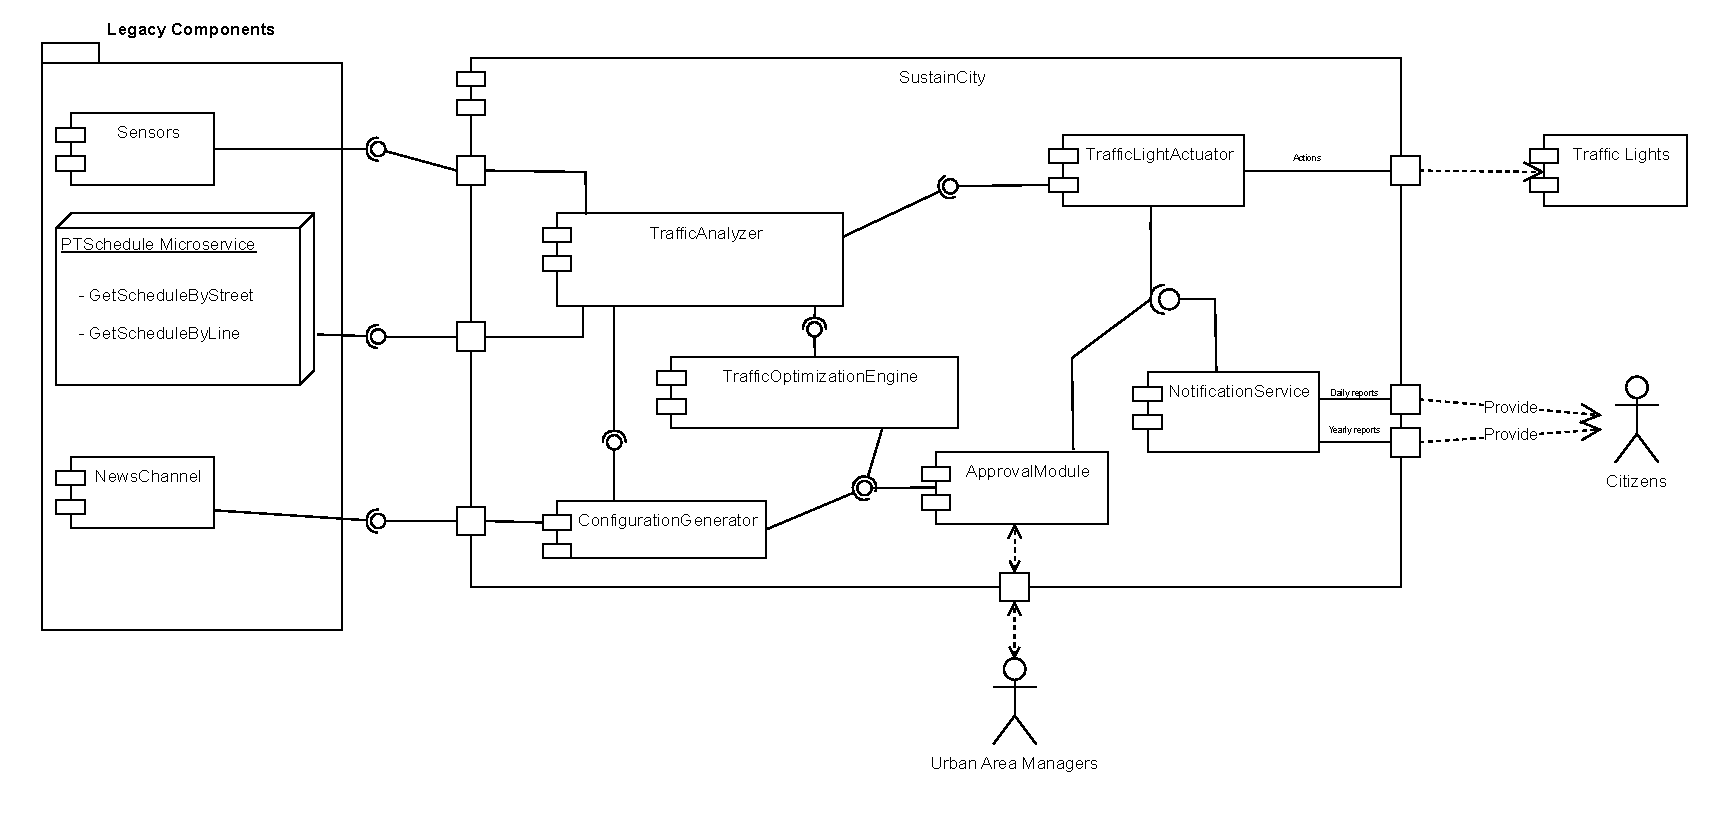
\includegraphics[width=1.1\textwidth]{diagrams/ComponentDiagram1.pdf}
    \caption{Component Diagram}
    \label{fig:ComponentDiagram.drawio}
\end{figure}


\newpage

\subsection{Sequence Diagrams}
In this section, we describe the sequence diagrams that visually represent the interactions and flow of events for the system’s key functionalities. 
These diagrams help illustrate how the system components collaborate to handle various use cases and scenarios.

\subsubsection{Traffic Light Sequence Diagram}
The \textbf{Traffic Light Sequence Diagram} shows how the system manages traffic lights in real time. 
\newline Sensors send new traffic data, and the \textit{TrafficAnalyzer} checks if changes are needed. If yes, it sends instructions to the \textit{TrafficLightActuator}, which updates the lights. 
The change is then confirmed and logged by the \textit{NotificationService}, which also prepares a traffic report.

\begin{figure}[h]
    \centering
    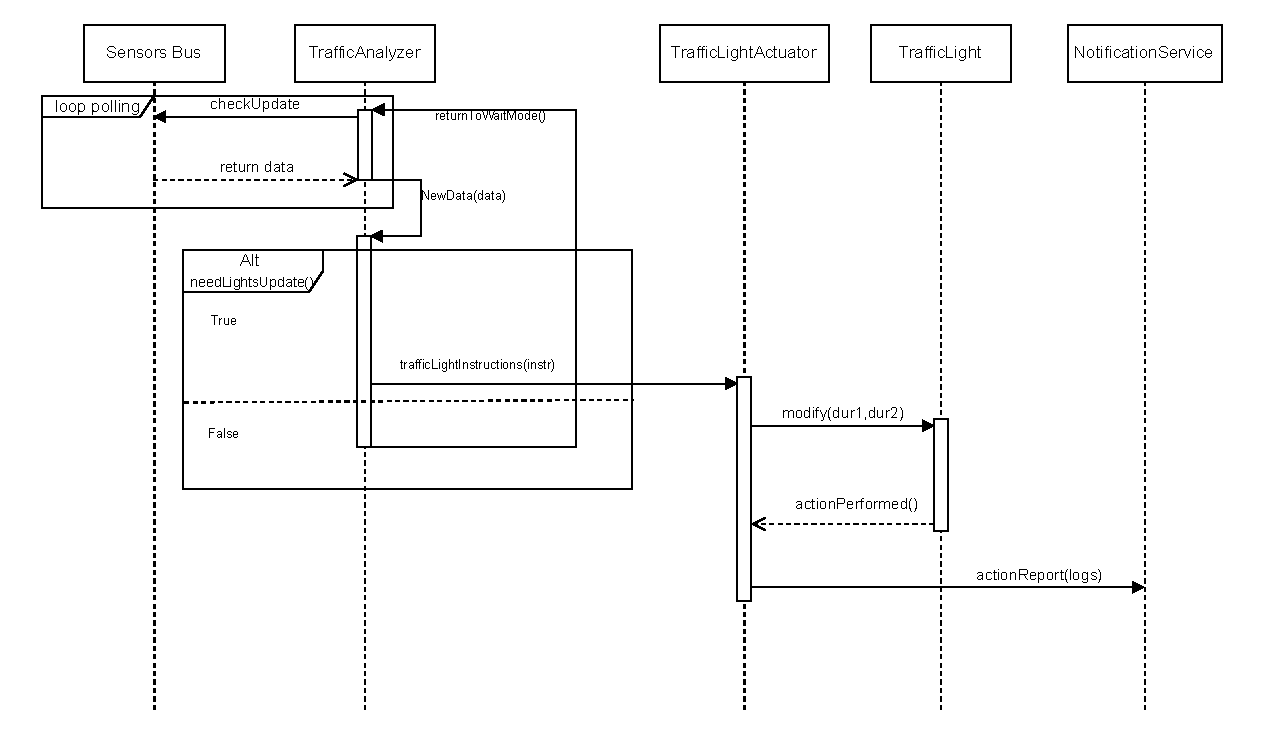
\includegraphics[width=1.1\textwidth]{diagrams/SequenceDiagram1.pdf}
    \caption{Type 1 Sequence Diagram}
    \label{fig:SeqDiag1.drawio}
\end{figure}

\newpage
\subsubsection{Traffic optimization Sequence Diagram}
The \textbf{Traffic Optimization Sequence Diagram} shows how the system uses traffic data to suggest improvements. 
\newline The \textit{TrafficAnalyzer} collects data and transport schedules, then sends them to the \textit{OptimizationEngine}, which creates suggestions. 
These are reviewed by \textit{Urban Area Managers} through the \textit{ApprovalModule}. The final decisions are logged and shared by the \textit{NotificationService}.
\begin{figure}[h]
    \centering
    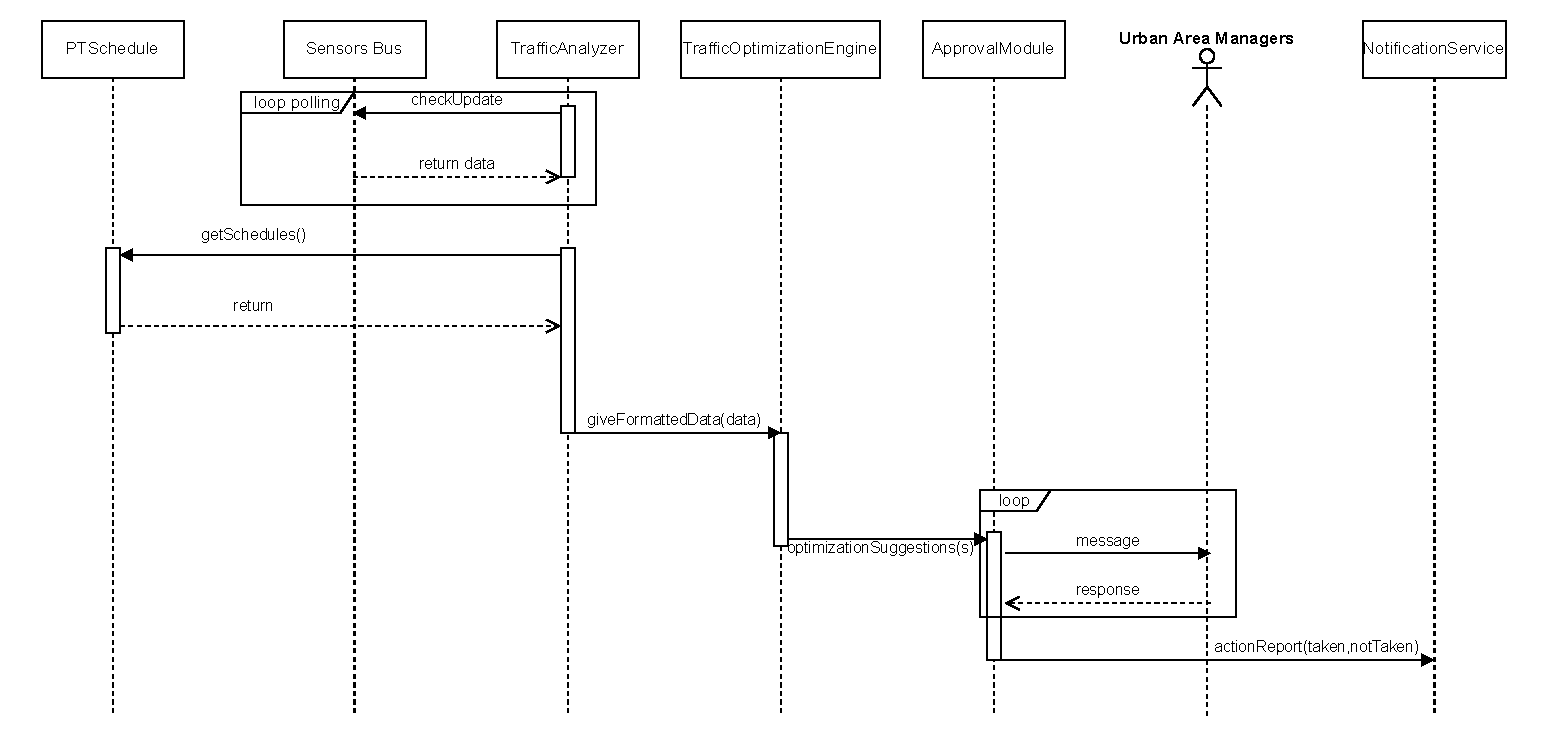
\includegraphics[width=1.1\textwidth]{diagrams/SequenceDiagram2.pdf}
    \caption{Type 2 Sequence Diagram}
    \label{fig:SeqDiag2.drawio}
\end{figure}

\subsubsection{Event-based configurations Sequence Diagram}
Sequence diagram for event-specific improvements to the urban area, very similar to the type 2 diagrams since the incapsulated logic
is the same.
\newline Here the \textit{TrafficAnalyzer} has the same connections with \textit{PTScheduleMicroservice and Sensors Bus}, but for redundancy reasons as been hide.
\begin{figure}[h]
    \centering
    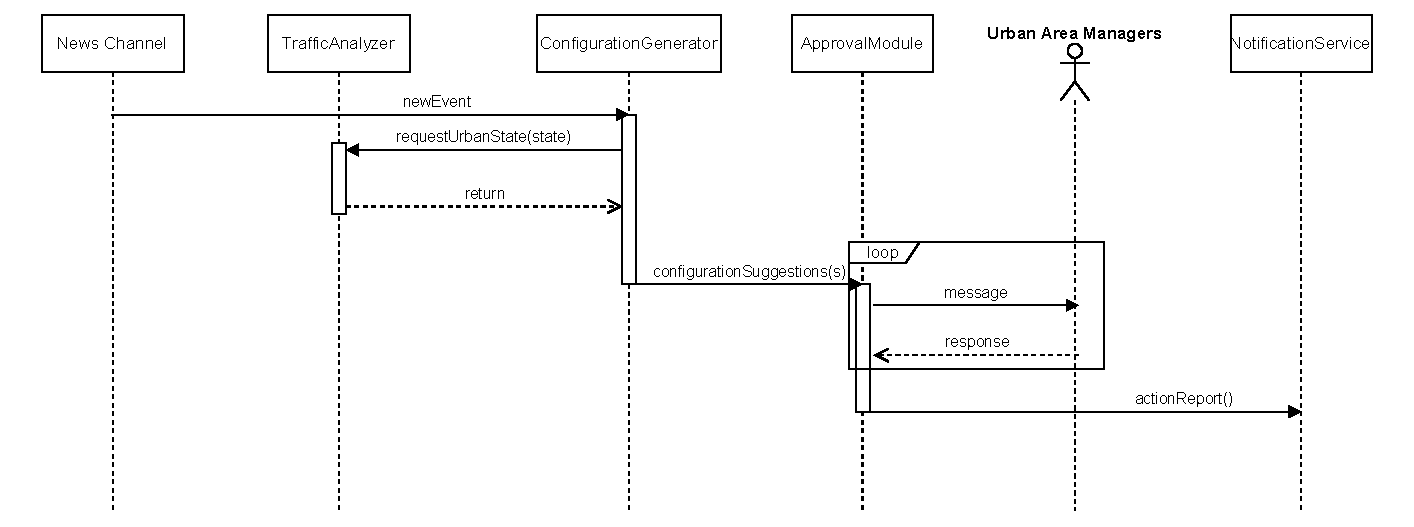
\includegraphics[width=1.1\textwidth]{diagrams/SequenceDiagram3.pdf}
    \caption{Type 3 Sequence Diagram}
    \label{fig:SeqDiag3.drawio}
\end{figure}
\newpage
\subsubsection{NotificationService Sequence Diagram}
The \textbf{Reporting Sequence Diagram} shows how the system generates and shares reports about traffic actions. 
\newline It collects logs from different modules, including \textit{TrafficLightActuator} and \textit{ApprovalModule}, and processes them through the \textit{NotificationService}. Daily reports are published for Type1 actions, while yearly summaries are created for Type2 and Type3. 
These reports are then made available on the \textit{Public Website} as required.
\begin{figure}[h]
    \centering
    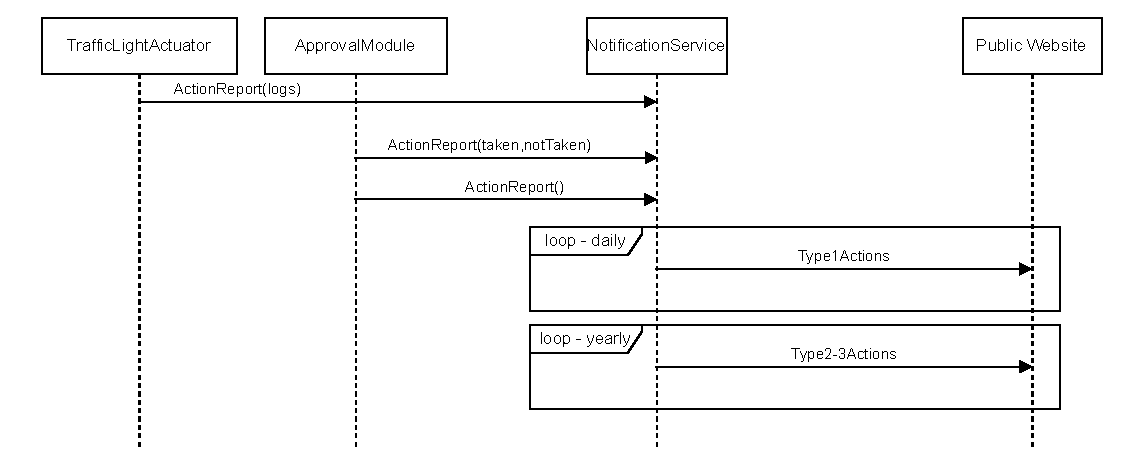
\includegraphics[width=1.1\textwidth]{diagrams/SequenceDiagram4.pdf}
    \caption{NotificationService Sequence Diagram}
    \label{fig:SeqDiag4.drawio}
\end{figure}

\newpage

\subsection{Critical points and design decisions}
\subsection*{Design decisions:}
The main component of this project is the TrafficAnalyzer module, by our design this module is the one in charge of retrieve the data 
about the urban area from outside and create a complex state with all these information.
This component will then provide the right data specifically formatted for other modules such as TrafficOptimizationEngine, ConfigurationGenerator and TrafficLightActuator, this choice is for 
allowing modularity and maintainability, so in case of a modification on the sensors or microservices output data the only component to be updated will be the
TrafficAnalyzer.
\newline Other design choice are:
\begin{itemize}
    \item TrafficOptimizationEngine receive data only from TrafficAnalyzer, the latter has the logic to encapsulate the right data while the optimizationEngine is only a compunting component that expect data in a particular format.
    \item Event-Driven Optimization: Unlike Type 2 actions (which focus on routine traffic improvements), Type 3 actions react dynamically to event-based disruptions.
    \item Approval Workflow: Ensures human oversight before implementing major transport reconfigurations, the ApprovalModule in particular can have some human workforce in order to keep the communication with the Urban Area Managers smooth.
    \item Public Engagement: Structured communication channels provide real-time notifications to affected commuters, as an example the channel was a public website, this component can be modified based on the administration choice.
\end{itemize}
\subsection*{Critical aspects:}
\begin{itemize}
    \item Event Data Accuracy: Must ensure data reliability from official event sources.
    \item Traffic Simulation Limitations: Forecasting congestion trends must balance real-time responsiveness and computational efficiency.
    \item Citizen Adaptability: The effectiveness of optimizations depends on commuter engagement with system-generated notifications.
\end{itemize}

\end{document}
